\documentclass[12pt]{beamer}
\usetheme{Berkeley}
\usepackage{graphicx}
\usepackage{booktabs}

\title{Jiskefet}

\author{Amin Chihab, Bastiaan Reinalda, Calvin Huynh, Misha Rigot, Ramon Gill}

\date{\today}

\begin{document}
	\begin{frame}
	\titlepage
	\end{frame}

	\begin{frame}{Table of contents}
		\tableofcontents
    \end{frame}
    
    \begin{frame}
        \frametitle{CERN trip}
   		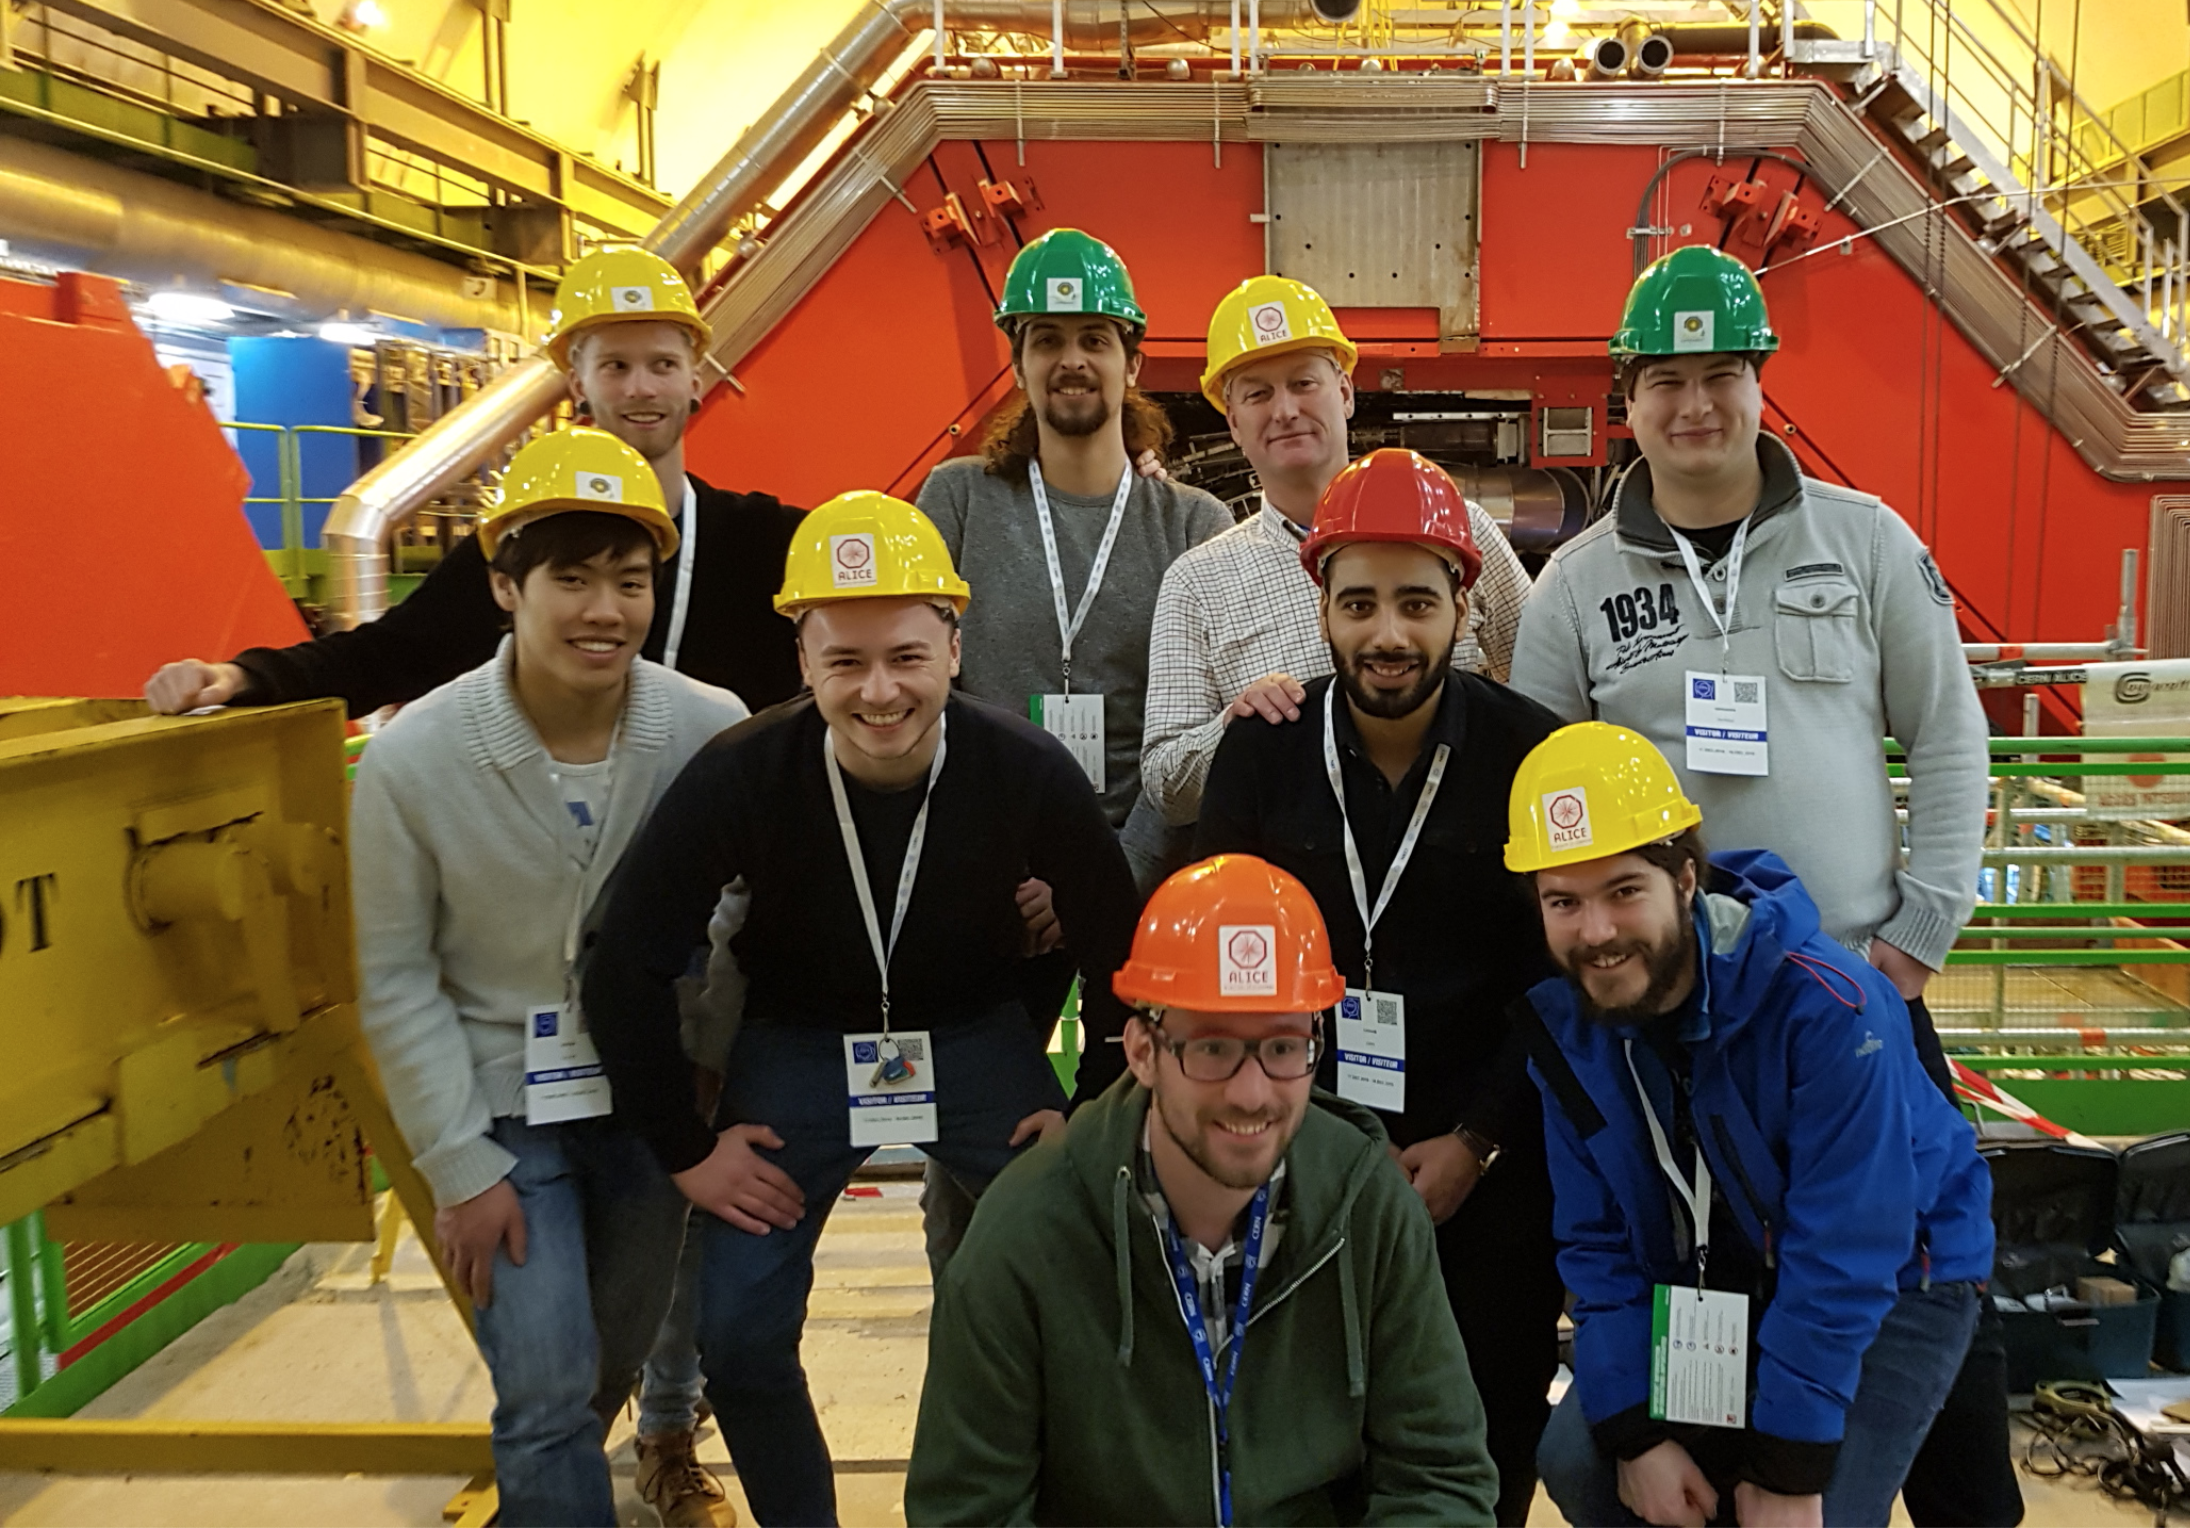
\includegraphics[scale=.25]{assets/cern-group.png}
    \end{frame}

    \section{Voortgang Jiskefet}
    \begin{frame}
        \frametitle{Huidige situatie}
        \begin{itemize}
            \item Version 0.1 released
            \item CERN SSO
            \item Logging
            \item Testing
            \item Jenkins CI
        \end{itemize}
    \end{frame}

    \begin{frame}
        \frametitle{Laatste sprint}
        \begin{itemize}
            \item General
            \begin{itemize}
                \item Config/environment variables validation
            \end{itemize}
            \item Front end
            \begin{itemize}
                \item Atomic design
                \item Redux
                \item Testing
            \end{itemize}
            \item Back end
            \begin{itemize}
                \item Standardize endpoints
                \item CERN SSO Logout
                \item More testing
            \end{itemize}
            \item Deployment
            \begin{itemize}
                \item Reduce the manual steps required to deploy the CI server
            \end{itemize}
        \end{itemize}
    \end{frame}

    \begin{frame}
        \frametitle{Demo}
        \href{http://dev-jiskefet.westeurope.cloudapp.azure.com/}{Demo link}
    \end{frame}

    \section{Scientific Programming}
    \begin{frame}
        \frametitle{Architecture \& Development}
    \end{frame}

    \begin{frame}
        \frametitle{Documentation}
        A Practical Method for Documenting Software Architectures
    \begin{itemize}
        \item Adopting a view-based approach to documentation,
        and then following that approach with discipline.
        \item Documentation in Git repository is done by adding a read.ME file
        per folder that needs explanation.
    \end{itemize}
    \end{frame}

    \begin{frame}
        \frametitle{Requirements}
    \end{frame}

    \begin{frame}
        \frametitle{Testing}
    \end{frame}
\end{document}